%%%%%%%%%%%%%%%%%%%%%%%%%%%%%%%%%%%%%%%%%%%%%%%%%%%%%%%%%%%
 \begin{frame}[fragile] \frametitle{Notes from Justin Grimmer}
Associate Professor\\Department of Political Science \\  Stanford University
\end{frame}

%\begin{frame}[fragile]
%\frametitle{Finding Lower Dimensional Embeddings of Text}
%\begin{itemize}
%\item[1)] Task:  
%\begin{itemize}
%\item[-] Embed our documents in a lower dimensional space
%\item[-] Visualize our documents
%\item[-] Inference about similarity
%\item[-] \alert{Social science inference about behavior} 
%\end{itemize}
%\item[2)] Objective Function, $f({X}, {\theta})$   
%\begin{itemize}
%\item[-] Reconstruction error: measure the distance between the \alert{embedded} points and the original points $\leadsto$ ${\theta}$ will contain basis vectors (\alert{principal components}) and \alert{weights} to those vectors   
%\item[-] Distance preservation: measure how well pairwise distances are preserved with distances $\leadsto$ ${\theta}$ a set of new lower-dimensional coordinates
%\end{itemize}
%\item[3)] Optimization $\leadsto$ eigenvectors, eigenvalues
%\begin{itemize}
%\item[-] Reconstruction error$\leadsto$ Search over components and weights 
%\item[-] Distance preservation$\leadsto$ Search over locations
%\end{itemize}
%\item[4)] Validation
%\begin{itemize}
%\item[a)] Labeling exercise: What are the dimensions? 
%\item[b)] Are the dimensions interesting semantically?
%\end{itemize}
%\end{itemize}
%
%
%\end{frame}


\begin{frame}[fragile]
\frametitle{An Introduction to Eigenvectors, Values, and Diagonalization}
\begin{defn}
Suppose ${A}$ is an $N \times N$ matrix and $\lambda$ is a scalar. 
\begin{eqnarray}
{A}{x} &= & \lambda {x} \nonumber 
\end{eqnarray}
Then ${x}$ is an \alert{eigenvector} and $\lambda$ is the associated \alert{eigenvalue}
\end{defn}

\end{frame}

\begin{frame}[fragile]
\frametitle{An Introduction to Eigenvectors, Values, and Diagonalization}
\begin{itemize}
\item[-] ${A}$ stretches the eigenvector ${x}$ 
\item[-] ${A}$ stretches ${x}$ by $\lambda$  
\item[-] To find eigenvectors/values: ({\tt eigen} in {\tt R} )  
\begin{itemize}
\item Find $\lambda$ that solves $\text{det}({A}- \lambda {I}) = 0 $ 
\item Find vectors in \alert{null space} of:  
\begin{eqnarray}
({A} - \lambda {I} ) &= & 0 \nonumber 
\end{eqnarray}
\end{itemize}
\end{itemize}
\end{frame}



\begin{frame}[fragile]
\frametitle{Finding a Lower Dimensional Space (Manifold Learning)}
\begin{center}
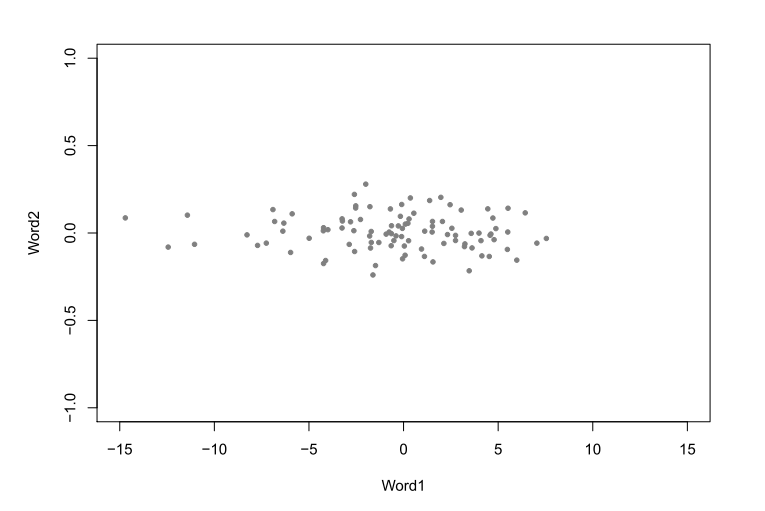
\includegraphics[width=0.8\linewidth,keepaspectratio]{PrCompExamp1}
\end{center}

\end{frame}

\begin{frame}[fragile]
\frametitle{Finding a Lower Dimensional Space (Manifold Learning)}
\begin{center}
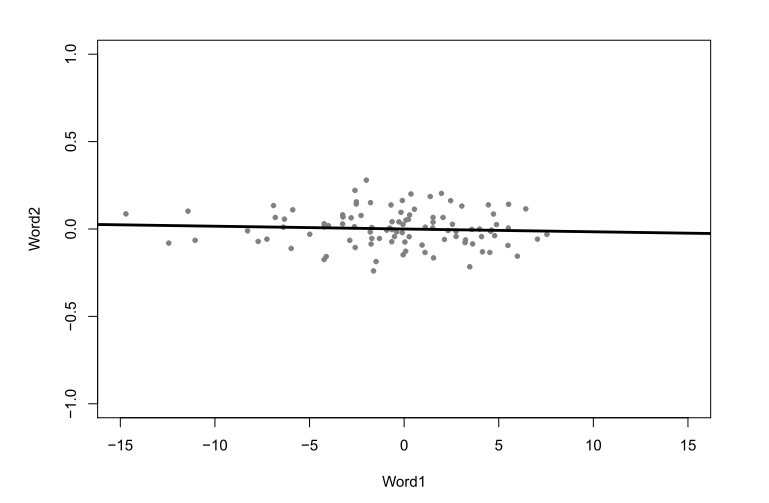
\includegraphics[width=0.8\linewidth,keepaspectratio]{PrCompExamp2}
\end{center}

\end{frame}


\begin{frame}[fragile]
\frametitle{Finding a Lower Dimensional Space (Manifold Learning)}
\begin{center}
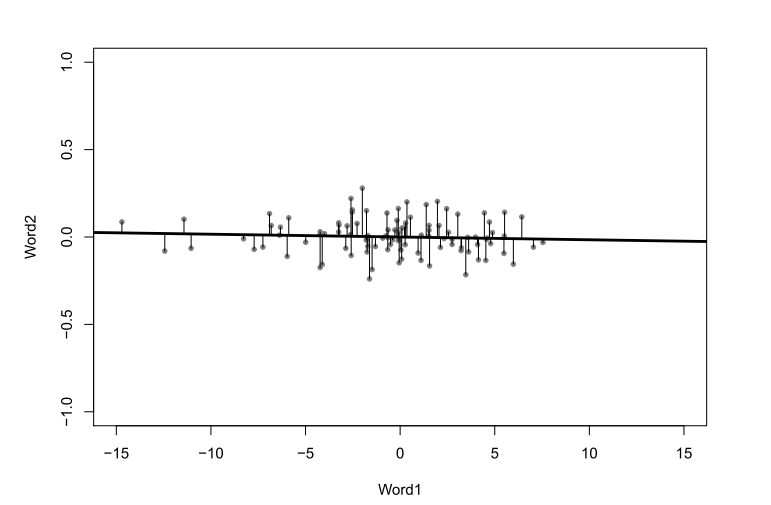
\includegraphics[width=0.8\linewidth,keepaspectratio]{PrCompExamp3}
\end{center}
\end{frame}


\begin{frame}[fragile]
\frametitle{Finding a Lower Dimensional Space (Manifold Learning)}
\begin{center}
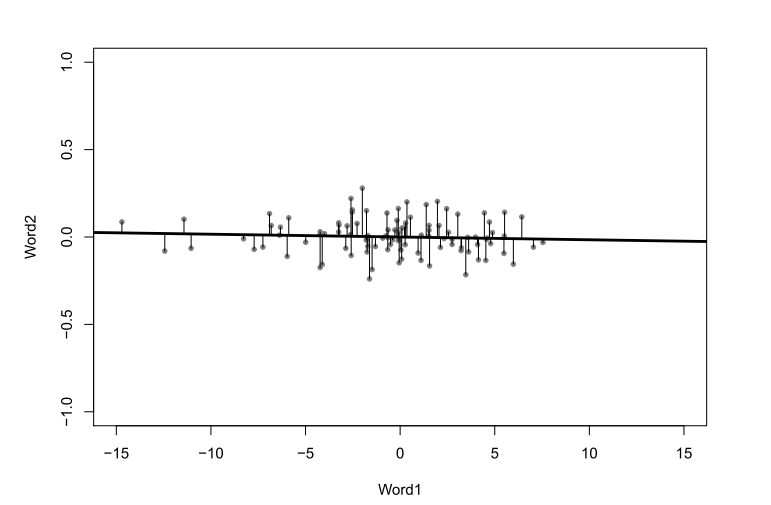
\includegraphics[width=0.3\linewidth,keepaspectratio]{PrCompExamp3}
\end{center}
Original data:
\begin{eqnarray}
{x}_{i} & = &  (x_{i1}, x_{i2}) \nonumber 
\end{eqnarray}

Which we approximate with  
\begin{eqnarray}
\tilde{{x}}_{i} & = & z_{i} {w}_{1} \nonumber \\
& =& z_{i} (w_{11}, w_{12}) \nonumber 
\end{eqnarray}
\end{frame}


\begin{frame}[fragile]
\frametitle{Finding a Lower Dimensional Space (Manifold Learning)}


\begin{center}
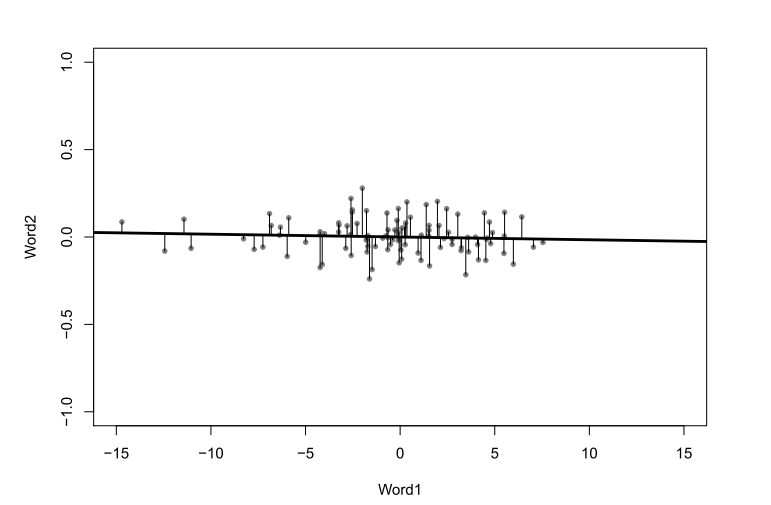
\includegraphics[width=0.3\linewidth,keepaspectratio]{PrCompExamp3}
\end{center}

Original data ${x}_{i} \in \Re^{J}$ 
\begin{eqnarray}
{x}_{i} & = & (x_{i1}, x_{i2}, \hdots, x_{iJ}) \nonumber 
\end{eqnarray}

Which we approximate with $L$($<J$) weights $z_{il}$ and vectors ${w}_{l} \in \Re^{J}$
\begin{eqnarray}
\tilde{{x}}_{i} & = & z_{i1} {w}_{1} + z_{i2} {w}_{2} + \hdots + z_{iL} {w}_{L} \nonumber 
\end{eqnarray}

Define ${\theta} = (\underbrace{{Z}}_{N \times L}, \underbrace{{W}_{L}}_{L \times J} )$ 


\end{frame}




\begin{frame}[fragile]
\frametitle{Principal Component Analysis$\leadsto$ Objective function}

Consider 1-dimensional case ($L = 1$), centered data, and $||{w}_{1}|| = 1$.  

\begin{eqnarray}
f({\theta},  {X}) & = & \frac{1}{N} \sum_{i=1}^{N} ||{x}_{i} - z_{i1}{w}_{1} ||^2     \nonumber \\
& = & \frac{1}{N} \sum_{i=1}^{N} ({x}_{i}  - z_{i1} {w}_{1} )^{'}({x}_{i}  - z_{i1} {w}_{1} ) \nonumber   \\
& = & \frac{1}{N}\sum_{i=1}^{N}\left({x}_{i}^{'}{x}_{i} - 2 z_{i1}{w}_{1}^{'}{x}_{i} + z_{i1}^{2} \right ) \nonumber  
\end{eqnarray}

${w}_{1}^{'}{w}_{1} = 1$ 
\end{frame}

\begin{frame}[fragile]
\frametitle{Principal Component Analysis$\leadsto$ Optimization}


Optimization:  
\begin{eqnarray}
\frac{\partial f({\theta}, {X})}{\partial z_{i1}}  & = &  - \frac{2 {w}_{1}^{'} {x}_{i} + 2 z_{i1}}{N} \nonumber \\
0 & = & - \frac{2 {w}_{1}^{'} {x}_{i} + 2 z_{i1}^{*}}{N} \nonumber \\  
z_{i1}^{*} & = & {w}_{1}^{'} {x}_{i} \nonumber 
\end{eqnarray}



\end{frame}





\begin{frame}[fragile]
\frametitle{Principal Component Analysis$\leadsto$ Optimization}
Substituting in $z_{i1}^{*}$  

\begin{eqnarray}
& = & \frac{1}{N} \sum_{i=1}^{N} ({x}_{i}  - z_{i1}^{*} {w}_{1} )^{'}({x}_{i}  - z_{i1}^{*} {w}_{1} ) \nonumber   \\
 & = & \frac{1}{N} \sum_{i=1}^{N} (\underbrace{{x}_{i}^{'}{x}_{i}}_{\text{Constant}}  - 2 z_{i1}^{*} \underbrace{{w}_{1}^{'}{x}_{i}}_{z_{i1}^{*}}  + \left(z_{i1}^{*}\right)^{2} \underbrace{{w}_{1}^{'}{w}_{1}}_{1} )   \nonumber   \\
 & = &  - \frac{1}{N} \sum_{i=1}^{N}   \left(z_{i1}^{*}\right)^{2} + c \nonumber   \\
 & = & - \frac{1}{N} \sum_{i=1}^{N} {w}_{1}^{'}{x}_{i}{x}^{'}_{i}{w}_{1} \nonumber   \\
 & = & -  {w}_{1}^{'}{\Sigma} {w}_{1} \nonumber
\end{eqnarray}



\end{frame}

\begin{frame}[fragile]
\frametitle{Principal Component Analysis$\leadsto$ Optimization}

\begin{eqnarray}
 & = & -  \sum_{i=1}^{N} {w}_{1}^{'}{\Sigma} {w}_{1} \nonumber  
\end{eqnarray}


where ${\Sigma}$ is the :  
\begin{itemize}
\item[-] Empirical covariance matrix$\leadsto \frac{1}{N} {X}^{'}{X}$ 
\item[-] \alert{Variance} of the projected data.  Define 
\begin{eqnarray}
{z}_{1} & = & ({w}_{1} {x}_{1}, {w}_{1} {x}_{2}, \hdots, {w}_{1}{x}_{N}) \nonumber \\ 
\text{var}({z}_{1}) & = & E[{z}_{1}^{2} ]  - E[{z}_{1}]^{2} \nonumber \\  
& = & \frac{1}{N} \sum_{i=1}^{N} z_{i1}^{2} - 0 \nonumber \\
& = & \frac{1}{N} \sum_{i=1}^{N} {w}_{1}^{'}{x}_{i}{x}_{i}^{'}{w}_{1} \nonumber 
\end{eqnarray}

\end{itemize}

Minimize reconstruction error $\leadsto$ maximize variance of projected data

\end{frame}


\begin{frame}[fragile]
\frametitle{Principal Component Analysis$\leadsto$ Optimization}

Maximize variance, subject to constraints  


\begin{eqnarray}
g({z}^{*}, {w}_{1}, {X}) & = & {w}_{1}^{'} {\Sigma}{w}_{1} - \lambda_{1}({w}_{1}^{'} {w}_{1} - 1 ) \nonumber \\
 \frac{\partial g({z}^{*}, {w}_{1}, {X})}{\partial {w}_{1}} &= & 2 {\Sigma}{w}_{1}  - 2 \lambda_{1} {w}_{1} \nonumber \\
 {\Sigma}{w}_{1}^{*} & = &  \lambda_{1} {w}_{1}^{*} \nonumber
\end{eqnarray}

$\alert{{w}_{1}^{*}}$ = \alert{Eigenvector of ${\Sigma}$}  (!!!!!!)  \\

We want ${w}_{1}$ to maximize variance and 

	\begin{eqnarray}
{w}_{1}^{'} {\Sigma} {w}_{1} = \lambda_{1} \nonumber 
	\end{eqnarray}

So ${w}_{1}$ is eigenvector associated with the largest eigenvalue $\lambda_{1}$ 

\end{frame}




\begin{frame}[fragile]
\frametitle{An Introduction to Eigenvectors, Values, and Diagonalization}


\begin{thm}
Suppose ${A}$ is an \alert{invertible} $N \times N$ matrix.  Then ${A}$ has $N$ distinct eigenvalues and $N$ linearly independent eigenvectors.  Further, we can write ${A}$ as, 

\begin{eqnarray}
{A} &= & {W}^{'}\begin{pmatrix}
\lambda_{1} & 0 & \hdots & 0 \\
0 & \lambda_{2} & \hdots & 0 \\
\vdots & \vdots & \ddots & \vdots \\
0 & 0&  \hdots & \lambda_{N}\\
\end{pmatrix}
{W} \nonumber 
\end{eqnarray}

where ${W} = \left({w}_{1}, {w}_{2}, \hdots, {w}_{N} \right)$ is an $N \times N$ matrix with the $N$ eigenvectors as column vectors.  

\end{thm}

\end{frame}


\begin{frame}[fragile]
\frametitle{An Introduction to Eigenvectors, Values, and Diagonalization}


\begin{defn}
Suppose $A$ is a covariance matrix.  Then, we can write $A$ as  

\begin{eqnarray}
{A} &= & {W}^{'}\begin{pmatrix}
\lambda_{1} & 0 & \hdots & 0 \\
0 & \lambda_{2} & \hdots & 0 \\
\vdots & \vdots & \ddots & \vdots \\
0 & 0&  \hdots & \lambda_{N}\\
\end{pmatrix}
{W} \nonumber 
\end{eqnarray}

Where $\lambda_{1}>\lambda_{2} > \hdots > \lambda_{N} \geq 0$. \\
We will call ${w}_{1}$ the first eigenvector, ${w}_{2}$ the second eigenvector, ..., ${w}_{j}$ the $\text{j}^{th}$ eigenvector.    

\end{defn}

\end{frame}


\begin{frame}[fragile]
\frametitle{Back to Principal Components}


\begin{thm}
Suppose we want to approximate $N$ observations ${x}_{i} \in \Re^{J}$ with $L < J$ orthogonal-unit length vectors ${w}_{l} \in \Re^{J}$ with associated scores $z_{il}$ to minimize reconstruction error:  

\begin{eqnarray}
f({X}, {\theta}) & = & \frac{1}{N} \sum_{i=1}^{N} || {x}_{i}  - \sum_{l = 1}^{L} z_{il} {w}_{l}||^{2} \nonumber
\end{eqnarray}

The optimal solution sets each ${w}_{l}$ to be the $l^{\text{th}}$ eigenvector of the empirical covariance matrix. Further $z_{il}^{*} = {w}_{l}^{'}{x}_{i}$ so that the $L$ dimensional representation is:
\begin{eqnarray}
{x}^{L}_{i} & = & ({w}_{1}^{'}{x}_{i}, {w}_{2}^{'}{x}_{i}, \hdots, {w}_{L}^{'}{x}_{i} ) \nonumber  
\end{eqnarray}

\end{thm}

\end{frame}



\begin{frame}[fragile]
\frametitle{Application of Principal Components in {\tt R}}

Consider press releases from 2005 US Senators  \\
Define ${x}_{i} = (x_{i1}, x_{i2}, \hdots, x_{iJ})$ as the rate senator $i$ uses $J$ words.  
\begin{eqnarray}
x_{ij} & = & \frac{\text{No. Times $i$ uses word $j$}}{\text{No. words $i$ uses}} \nonumber
\end{eqnarray}

{\tt  dtm}: $100 \times 2796$ matrix containing word rates for senators\\  
{\tt prcomp(dtm) } applies principal components


\end{frame}


\begin{frame}[fragile]
\frametitle{Application of Principal Components in {\tt R}}
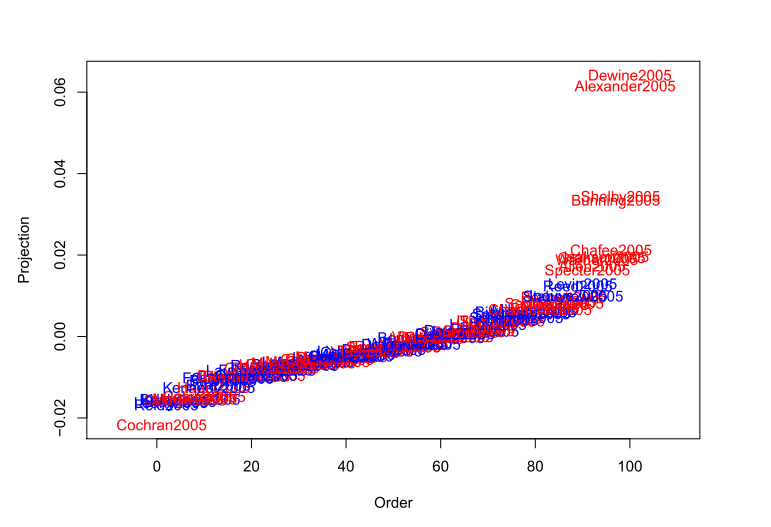
\includegraphics[width=0.8\linewidth,keepaspectratio]{FirstPrinComp}
\end{frame}

\begin{frame}[fragile]
\frametitle{Application of Principal Components in {\tt R}}
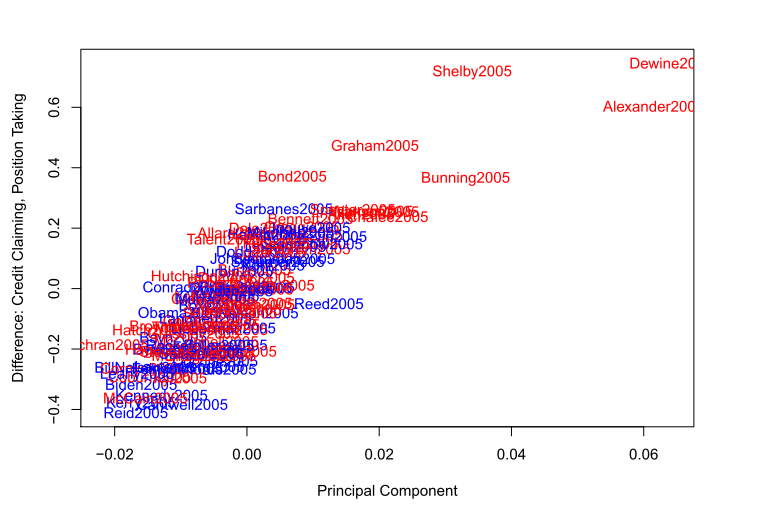
\includegraphics[width=0.8\linewidth,keepaspectratio]{CreditClaimPrinComp}
\end{frame}


\begin{frame}[fragile]
\frametitle{How do we select the number of dimensions $L$?$\leadsto$ \alert{Model}}

We want to minimize reconstruction error  $\leadsto$ how well did we do?  \\

\begin{eqnarray}
\text{error}(L) & = & \frac{1}{N} \sum_{i=1}^{N} ||{x}_{i} - \sum_{l = 1}^{L} z_{il} {w}_{l} ||^{2}   \nonumber 
\end{eqnarray}

Simplifying:  
\begin{eqnarray}
\text{error}(L)  & = & \frac{1}{N} \sum_{i=1}^{N} ({x}_{i} - \sum_{l = 1}^{L} z_{il}{w}_l)^{'} ({x}_{i} - \sum_{l = 1}^{L} z_{il}{w}_l ) \nonumber \\
& = & \frac{1}{N} \sum_{i=1}^{N} \left({x}_{i}^{'}{x}_{i} - \sum_{l=1}^{L} z_{il}^{2} \right)\nonumber
\end{eqnarray}

\end{frame}

\begin{frame}[fragile]
\frametitle{How do we select the number of dimensions $L$?$\leadsto$ \alert{Model}}

Four types of terms:  
\begin{itemize}
\item[1)] ${x}_{i}^{'}{x}_{i} $
\item[2)] $z_{ij}z_{ik} {w}_{j}^{'}{w}_{k} = z_{ij}z_{ik} 0  = 0 $  
\item[3)] $z_{ij}z_{ij} {w}_{j}^{'}{w}_{j} = z_{ij}^2$ 
\item[4)] ${x}_{i}^{'}\sum_{l=1}^{L} z_{il} {w}_{l} = \sum_{l=1}^{L} z_{il}^{2} $
\end{itemize}
\end{frame}


\begin{frame}[fragile]
\frametitle{How do we select the number of dimensions $L$?$\leadsto$ \alert{Model}}
\begin{small}
\begin{eqnarray}
\text{error}(L) & = & \frac{1}{N} \sum_{i=1}^{N} \left({x}_{i}^{'}{x}_{i} - \sum_{l=1}^{L} z_{il}^{2} \right)\nonumber  \\
& = & \frac{1}{N} \sum_{i=1}^{N} \left({x}_{i}^{'}{x}_{i} - \sum_{l=1}^{L} {w}_{l} {x}_{i} {x}_{i}^{'}{w}_{l} \right) \nonumber  \\
& = & \frac{1}{N} \sum_{i=1}^{N} \left({x}_{i}^{'}{x}_{i}\right)  - \frac{1}{N} \sum_{l=1}^{L} \sum_{l=1}^{N} {w}_{i}^{'}{x}_{i} {x}_{i}^{'} {w}_{i} \nonumber  \\
& = & \frac{1}{N} \sum_{i=1}^{N} \left({x}_{i}^{'}{x}_{i}\right)  - \sum_{l=1}^{L} {w}_{l}^{'} {\Sigma} {w}_{l}  \nonumber  \\
& = & \frac{1}{N} \sum_{i=1}^{N} \left({x}_{i}^{'}{x}_{i}\right) - \sum_{l=1}^{L} \lambda_{l} {w}_{l}^{'}{w}_{l} \nonumber   \\
& = & \frac{1}{N} \sum_{i=1}^{N} \left({x}_{i}^{'}{x}_{i}\right) - \sum_{l=1}^{L} \lambda_{l} \nonumber  
\end{eqnarray}
\end{small}
\end{frame}


\begin{frame}[fragile]
\frametitle{How do we select the number of dimensions $L$?$\leadsto$ \alert{Model}}


If $L = J$  
\begin{eqnarray}
\text{error}(J) & = & \frac{1}{N} \sum_{i=1}^{N} \left({x}_{i}^{'}{x}_{i}\right) - \sum_{l=1}^{J} \lambda_{l} = 0 \nonumber   
\end{eqnarray}

So for $L < J$, 

\begin{eqnarray}
0  & = & \frac{1}{N} \sum_{i=1}^{N} \left({x}_{i}^{'}{x}_{i}\right) - (\sum_{l=1}^{L} \lambda_{l} + \sum_{j=L+1}^{J} \lambda_{l} ) \nonumber \\  
\sum_{j=L+1}^{J} \lambda_{l}  & = & \frac{1}{N} \sum_{i=1}^{N} \left({x}_{i}^{'}{x}_{i}\right) - \sum_{l=1}^{L} \lambda_{l} \nonumber \\  
\sum_{j=L+1}^{J} \lambda_{l}  & = & \text{error}(L) \nonumber 
\end{eqnarray}


\end{frame}


\begin{frame}[fragile]
\frametitle{How do we select the number of dimensions $L$?$\leadsto$ \alert{Model}}

\begin{eqnarray}
\sum_{j=L+1}^{J} \lambda_{l}  & = & \text{error}(L) \nonumber   
\end{eqnarray}

\begin{itemize}
\item[-] Error = Sum of ``remaining" eigenvalues
\item[-] Total variance explained =  (sum of included eigenvalues)/(sum of all eigenvalues) 
\end{itemize}
Recommendation$\leadsto$ look for Elbow 
\end{frame}

\begin{frame}[fragile]
\frametitle{How do we select the number of dimensions $L$?$\leadsto$ \alert{Model}}
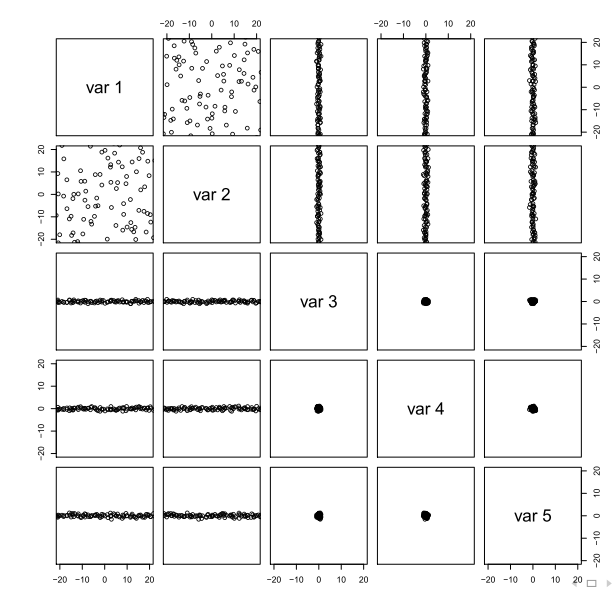
\includegraphics[width=0.6\linewidth,keepaspectratio]{ToyExamplePlot}
\end{frame}


\begin{frame}[fragile]
\frametitle{How do we select the number of dimensions $L$?$\leadsto$ \alert{Model}}
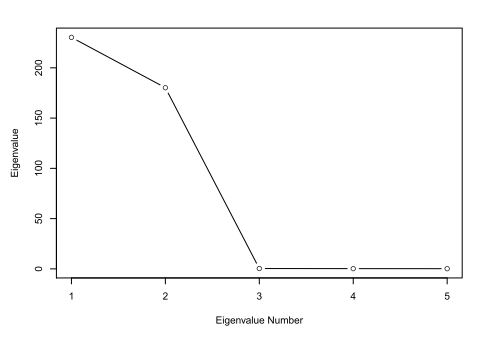
\includegraphics[width=0.8\linewidth,keepaspectratio]{EigenPlot1}
\end{frame}


\begin{frame}[fragile]
\frametitle{How do we select the number of dimensions $L$?$\leadsto$ \alert{Model}}
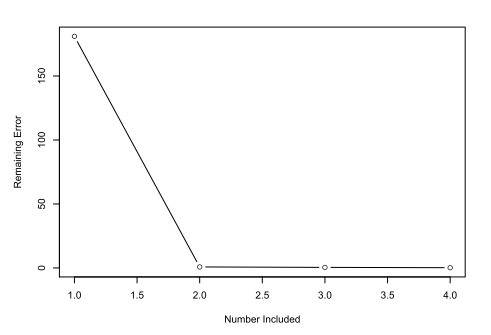
\includegraphics[width=0.8\linewidth,keepaspectratio]{EigenPlot2}
\end{frame}



\begin{frame}[fragile]
\frametitle{How do we select the number of dimensions $L$?$\leadsto$ \alert{Model}}
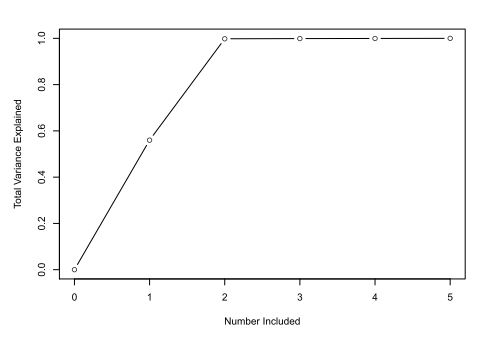
\includegraphics[width=0.8\linewidth,keepaspectratio]{EigenPlot3}
\end{frame}

\begin{frame}[fragile]
\frametitle{Non-model based evaluations: What's the point?}

What is the true underlying dimensionality of ${X}$? \alert{J}(!!!!!)  \\

\begin{itemize}
\item[-] Attempts to assess dimensionality require a \alert{model}$\leadsto$ some way to tradeoff accuracy of reconstruction with simplicity
\item[-] \alert{Any} answer (no matter how creatively obtained) supposes \alert{you have the right function to measure tradeoff}
\item[-] The ``right" number of dimensions depends on the \alert{task} you have in mind
\end{itemize}


{\large Mathematical model$\leadsto$ insufficient to make modeling decision} 

\end{frame}



\begin{frame}[fragile]
\frametitle{Kernel Principal Component Analysis}
Recall from Thursday that we define a \alert{Kernel} ($N \times N$) matrix as:
\begin{eqnarray}
{K} & = & \begin{pmatrix}
k({x}_{1}, {x}_{1}) & k({x}_{1}, {x}_{2}) & \hdots & k({x}_{1}, x_{N}) \\
k({x}_{2}, {x}_{1}) & k({x}_{2}, {x}_{2}) & \hdots & k({x}_{2}, {x}_{N}) \\
\vdots & \vdots & \ddots & \vdots \\
k({x}_{N}, {x}_{1}) & k({x}_{N}, {x}_{2}) & \hdots & k({x}_{N}, {x}_{N}) \\
\end{pmatrix}\nonumber 
\end{eqnarray}
 
Where we suppose this matrix emerges from applying $\phi: \Re^{J} \rightarrow \Re^{M}$ to the data and then taking the inner product:  
\begin{eqnarray}
{K} & = & {\Phi}{\Phi}^{'} \text{ (The inner product matrix)} \nonumber \\
& = & \begin{pmatrix}
\phi({x}_{1})^{'}\phi({x}_{1}) & \phi({x}_{1})^{'}\phi({x}_{2}) & \hdots & \phi({x}_{1})^{'}\phi({x}_{N}) \nonumber \\
\phi({x}_{2})^{'}\phi({x}_{1}) & \phi({x}_{2})^{'}\phi({x}_{2}) & \hdots & \phi({x}_{2})^{'}\phi({x}_{N})\\
\vdots & \vdots & \ddots & \vdots \\
\phi({x}_{N})^{'}\phi({x}_{1}) & \phi({x}_{N})^{'}\phi({x}_{2}) & \hdots & \phi({x}_{N})^{'}\phi({x}_{N}) \\
\end{pmatrix} \nonumber 
\end{eqnarray}
\alert{Compute PCA of ${\Phi}$ from ${\Phi}{\Phi}^{'}$ }
\end{frame}


\begin{frame}[fragile]
\frametitle{Kernel PCA}

PCA of ${X}$ Eigenvectors of ${X}^{'}{X}$ ($\frac{1}{N}$ doesn't affect eigenvectors)  \\
Suppose ${u}_{1}$ is an eigenvector for ${X}{X}^{'}$, with value $\lambda_{1}$.   Then   
\begin{eqnarray}
({X}{X}^{'}){u}_{1} & = & \lambda_{1} {u}_{1} \nonumber \\ 
({X}^{'}{X}) ({X}^{'} {u}_{1})  & = & \lambda_{1} ({X}^{'}{u}_{1}) \nonumber \\ 
 & = & \lambda_{1} {v}_{1} \nonumber
\end{eqnarray}

But ${v}_{1}$ needs unit length, and  
\begin{eqnarray}
||{v}_{1}||^{2}  = {v}^{'}_{1} {v}_{1}  \nonumber \\
& = & {u}_{1}^{'}{X}{X}^{'}{u}_{1} \nonumber \\ 
& = & \lambda_{1} {u}_{1}^{'}{u}_{1} = \lambda_{1}  \nonumber 
\end{eqnarray}

So first eigenvector of ${X}^{'}{X}$ is 
\begin{eqnarray}
{w}_{1} & = & \frac{1}{\sqrt{\lambda_{1}} } {X}^{'}{u}_{1} \nonumber
\end{eqnarray}

\end{frame}

\begin{frame}[fragile]
\frametitle{Kernel PCA}

${K} = {\Phi}{\Phi}^{'}$ (assume ${\Phi}$ is mean-centered, for now)  \\

We can obtain ${u}_{1}$ and $\lambda_{1}$ from ${K}$.  We know that 
\begin{eqnarray}
{w}_{1} & = & \frac{1}{\sqrt{\lambda_{1}}} \underbrace{{\Phi}^{'}}_{\text{Unknown}} {u}_{1} \nonumber 
\end{eqnarray}

But suppose we want to project a point $\phi({x}_{i})$, then  
\begin{eqnarray} 
\phi({x}_{i})^{'}{w}_{1}  &= & \frac{1}{\sqrt{\lambda_{1}}} \phi({x}_{i})^{'} {\Phi}^{'} {u}_{1} \nonumber \\
\phi({x}_{i})^{'} {\Phi}^{'} & = & \left[\phi({x}_{i} )^{'}\phi({x}_{1}), \phi({x}_{i} )^{'}\phi({x}_{2}), \hdots, \phi({x}_{i} )^{'}\phi({x}_{N}) \right] \nonumber \\
 &  = & \left[k({x}_{i}, {x}_{1}) , k({x}_{i}, {x}_{2}) , \hdots, k({x}_{i}, {x}_{N}) \right] = {k}({x}_{i}, * ) \nonumber 
\end{eqnarray}

Then, we can obtain projection for observation $i$ using Kernel with
\begin{eqnarray}
\phi({x}_{i})^{'} {w}_{1} & = & \frac{1}{\sqrt{\lambda_{1}}} {k}({x}_{i}, *) {u}_{1} \nonumber 
\end{eqnarray}


\end{frame}

\begin{frame}[fragile]
\frametitle{Kernel PCA}

Center ${K}$?\\

Use centering matrix ${H}$
\begin{eqnarray}
{H}  & = & {I}_{N}  - \frac{({1}_{N} {1}_{N}^{'})}{N} \nonumber \\
{K}_{\text{center}} & = & {H} {K} {H} \nonumber 
\end{eqnarray}



\end{frame}




\begin{frame}[fragile]
\frametitle{Spirling and Indian Treaties}


\alert{Spirling (2013)}: model Treaties between US and Native Americans  \\
Why?
\begin{itemize}
\item[-] American political development
\item[-] IR Theories of Treaties and Treaty Violations
\item[-] Comparative studies of indigenous/colonialist interaction 
\item[-] \alert{Political Science question}: how did Native Americans lose land so quickly?
\end{itemize}


\end{frame}


\begin{frame}[fragile]
\frametitle{Spirling and Indian Treaties}


How do we preserve word order and semantic language?  \\

After stemming, stopping, bag of wording:   
\begin{itemize}
\item[-] {\tt Peace Between Us}  
\item[-] {\tt No Peace Between Us} 
\end{itemize}
  
 are identical.  \\
 
 Spirling uses complicated representation of texts to preserve word order $\leadsto$ broad application\\ 
\tt \alert{Peac}e Between Us
\tt P\alert{eace} Between Us 
\tt Pe\alert{ace }Between Us
\tt Pea\alert{ce B}etween Us
\tt Peac\alert{e Be}tween Us
\tt Peace\alert{ Bet}ween Us
\tt Peace \alert{Betw}een Us
\tt Peace B\alert{etwe}en Us
\tt Peace Be\alert{twee}n Us
\tt Peace Bet\alert{ween} Us 
\tt Peace Betw\alert{een }Us
\tt Peace Betwe\alert{en U}s
\tt Peace Betwee\alert{n Us}





\end{frame}

\begin{frame}[fragile]
\frametitle{Spirling and Indian Treaties}

Consider documents ${x}_{i}$ and ${x}_{j}$, where we have preserved order, punctuation, and all else.  \\
We say ${x}_{i} \in \mathcal{X}$  \\
Spirling examines $5$-character strings, $s \in \mathcal{A}$  \\
Define:  \\
$\phi_{s}:\mathcal{X}\rightarrow\Re$ as a function that counts the number of times string $s$ occurs in document ${x}$.\\ 

Define \alert{string kernel} to be, 
\begin{eqnarray}
k({x}_{i}, {x}_{j} ) & = & \sum_{s \in \mathcal{A}} w_{s} \phi_{s}({x}_{i})\phi_{s}({x}_{j}) \nonumber 
\end{eqnarray}

${\phi}({x}_{i}) \approx {{32}\choose{5}}$ element long count vector


\end{frame}

\begin{frame}[fragile]
\frametitle{Spirling and Indian Treaties}

\begin{center}
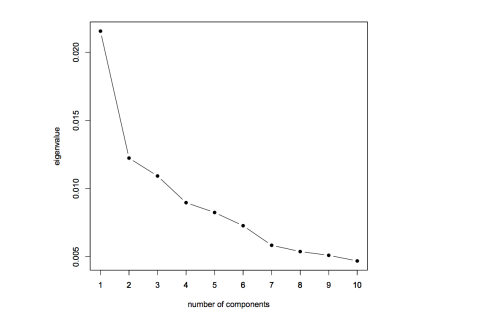
\includegraphics[width=0.8\linewidth,keepaspectratio]{Scree}
\end{center}


\end{frame}

\begin{frame}[fragile]
\frametitle{Spirling and Indian Treaties}

\begin{center}
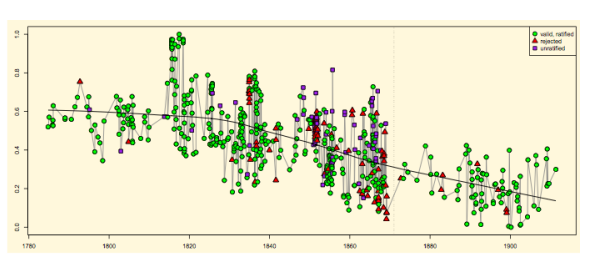
\includegraphics[width=0.8\linewidth,keepaspectratio]{HarshFig}
\end{center}


\end{frame}



\begin{frame}[fragile]
\frametitle{Classic Multidimensional Scaling$\leadsto$ Objective Function}

Suppose we have an $N \times N$ matrix ${D}\leadsto$  matrix of squared Euclidean distances between documents ${x}_{i}, {x}_{j}  \in \Re^{J}$.  \\

Typical distance between ${x}_{i}$ and ${x}_{j}$  

\begin{eqnarray}
d_{ij}^{2} & = & \sum_{k=1}^{J} (x_{ik} - x_{jk})^{2} \nonumber 
\end{eqnarray}

For all $N$ documents we look for points ${z}_{i} \in \Re^{L}$ (with $L < J$ ) to minimize 
\begin{eqnarray}
f({X}, {\theta}) & = & f({X}, {Z}) \nonumber \\
 & =& \sum_{i\neq j} \left(d_{ij} - ||z_{i} - z_{j}|| \right)^{2} \nonumber  
\end{eqnarray}

\alert{Recover best low-dimensional representation}$\leadsto$ Eigenvector decomposition of ${D}$

\end{frame}


\begin{frame}[fragile]
\frametitle{Classic Multidimensional Scaling$\leadsto$ Optimization}

\begin{itemize}
\item[1)] Start with ${D}$ \\
\item[2)] ``Center" ${D}$ to obtain ${X}{X}^{'}$
\item[3)] Find largest eigenvectors of ${X}{X}^{'}$
\end{itemize}

\end{frame}


\begin{frame}[fragile]
\frametitle{Classic Multidimensional Scaling$\leadsto$ Optimization}

Center the distance matrix, obtain inner product 
\begin{eqnarray}
d_{ij}^{2} &= & \sum_{k=1}^{J} (x_{ik} - x_{jk})^{2} \nonumber \\
 &= & \sum_{k=1}^{J} (x_{ik}^2 - 2x_{ik} x_{jk} + x_{jk}^{2} ) \nonumber \\
 & = & \underbrace{{x}_{i}^{'}{x}_{i}}_{\text{rows}} - 2 {x}_{i} {x}_{j} + \underbrace{{x}_{j}^{'}{x}_{j}}_{\text{columns}} \nonumber 
\end{eqnarray}

\begin{itemize}
\item[-] Subtract off row means 
\item[-] Subtract off column means
\item[-] Divide by -2
\end{itemize}

\begin{eqnarray}
{X}{X}^{'} & = & \frac{-{H}{D}{H} \nonumber }{2}
\end{eqnarray}

\end{frame}


\begin{frame}[fragile]
\frametitle{Classic Multidimensional Scaling$\leadsto$ Optimization}

We can write ${X}{X}^{'}$ as

\begin{eqnarray}
{X}{X}^{'} & = & {W}^{'}\begin{pmatrix}
\lambda_{1} & 0 & \hdots &  0 \\
0 & \lambda_{2} & \hdots & 0 \\
\vdots  & \vdots & \ddots & \vdots \\
0 & 0 & \hdots & \lambda_{N} \\
\end{pmatrix} {W} \nonumber \\
& = & \underbrace{{W}^{'} \begin{pmatrix}
\sqrt{\lambda_{1}} & 0 & \hdots &  0 \\
0 & \sqrt{\lambda_{2}} & \hdots & 0 \\
\vdots  & \vdots & \ddots & \vdots \\
0 & 0 & \hdots & \sqrt{\lambda_{N}} \\
\end{pmatrix}}_{{X}} \underbrace{\begin{pmatrix}
\sqrt{\lambda_{1}} & 0 & \hdots &  0 \\
0 & \sqrt{\lambda_{2}} & \hdots & 0 \\
\vdots  & \vdots & \ddots & \vdots \\
0 & 0 & \hdots & \sqrt{\lambda_{N}} \\
\end{pmatrix} {W}}_{{X}^{'}} \nonumber 
\end{eqnarray}

Approximate ${X}$ with first $L$ eigenvectors


\end{frame}


\begin{frame}[fragile]
\frametitle{Classic Multidimensional Scaling$\leadsto$ Optimization}

Define ${z}_{i}  \in \Re^{L}$ as, 
\begin{eqnarray}
{z}_{i}^{*} & = & \left(\sqrt{\lambda_{1}}w_{1i},\sqrt{\lambda_{2}}w_{2i}, \hdots, \sqrt{\lambda_{L}} w_{Li} \right) \nonumber 
\end{eqnarray}

 

\begin{itemize}
\item[-] Same diagnostics as before: eigenvalues
\item[-] Same issues in dimension reduction$\leadsto$ what are the dimensions for your task
\item[-] Information up to \alert{rotation} and arbitrary \alert{center} (same result with any \alert{orthogonal} matrix ${M}$)
\end{itemize}


\end{frame}



\begin{frame}[fragile]
\frametitle{Comparing MDS and PCA}
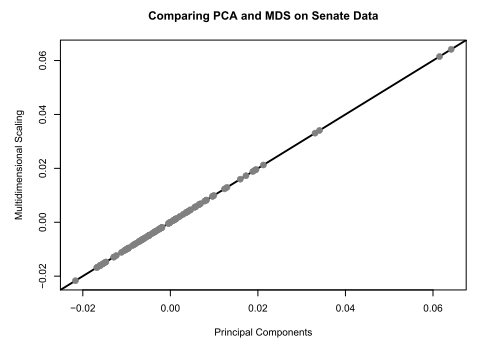
\includegraphics[width=0.8\linewidth,keepaspectratio]{PCAvsMDS}
\end{frame}

\begin{frame}[fragile]
\frametitle{Comparing MDS and PCA}
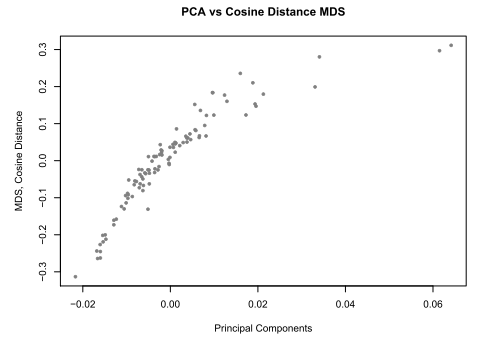
\includegraphics[width=0.8\linewidth,keepaspectratio]{PCAvsMDS2}
\end{frame}

\begin{frame}[fragile]
\frametitle{Comparing MDS and PCA}
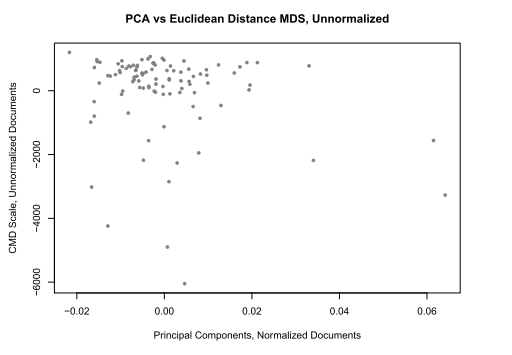
\includegraphics[width=0.8\linewidth,keepaspectratio]{PCAvsMDS3}
\end{frame}
%
%
%
%\begin{frame}[fragile]
%\frametitle{Sammon Multidimensional Scaling$\leadsto$ Manifold Learning}
%
%Many other methods we won't cover:  
%
%\begin{itemize}
%\item[-] Sammon Multidimensional Scaling$\leadsto$ prioritizes small differences 
%\begin{eqnarray}
%f({X}, {Z}) & = & \sum_{i\neq j} \frac{ (d_{ij}  - ||z_{i} - z_{j}||)^{2}  }{d_{ij} } \nonumber 
%\end{eqnarray}
%\item[-] \alert{Landmark MDS}$\leadsto$ for large scale embeddings
%\item[-] \alert{ISOMap}$\leadsto$ Non-linear embedding, emphasizing local patterns
%\end{itemize}
%
%
%
%\begin{itemize}
%\item[1)] Calculate distance matrix
%\item[2)] Create $K$ nearest neighbor graph: find $K$ nearest neighbors for each point, with edge weight = Euclidean distance
%\item[3)] Compute shortest weighted path between each node (distance matrix)
%\item[4)] Apply classic MDS
%\end{itemize}
%
%
%Common theme$\leadsto$ Manifold Learning
%
%         
%
%\end{frame}
%
%
%
%
%
%
%\begin{frame}[fragile]
%\frametitle{Low Dimensional Embedding}
%
%
%\begin{itemize}
%\item[1)] Find lower dimensional space to summarize documents$\leadsto$ Eigenvectors
%\item[2)] Thursday: basic language models and the Dirichlet distribution
%\end{itemize}
%
%
%\end{frame}
